\section{Confirmatory simulation protocol and complete evidence ledger}

\subsection{Design, sequential rule and estimands}
The Stage II design identifier and its SHA-256 hash are frozen in \path{simulation/configs/stage_ii_confirmatory.yaml}. Experiments E1--E6 each define their factors, contrasts, binary or continuous estimands, family-wise coverage, multiplicity, sequential check points, precision targets and maximum replication count. The execution writes \SimulationRawRows{} raw result rows, \SimulationContrasts{} contrast rows, \SimulationScenarios{} scenario-registry rows, optimal-face audits, frontier records, dependence diagnostics, information cells and attribution coalitions.

At each registered check, continuous intervals use the frozen family-wise $t$ critical value and binary intervals use the registered family-wise rule. An experiment stops for precision only when all primary intervals pass. Otherwise it proceeds to the next checkpoint until the maximum is reached. The evidence status is assigned mechanically from the complete experiment, not from selected contrasts. E2 and E6 stop at $n=16$ with precision achieved. E1, E3, E4 and E5 reach $n=64$ and fail.

\begin{figure}[t]
\centering
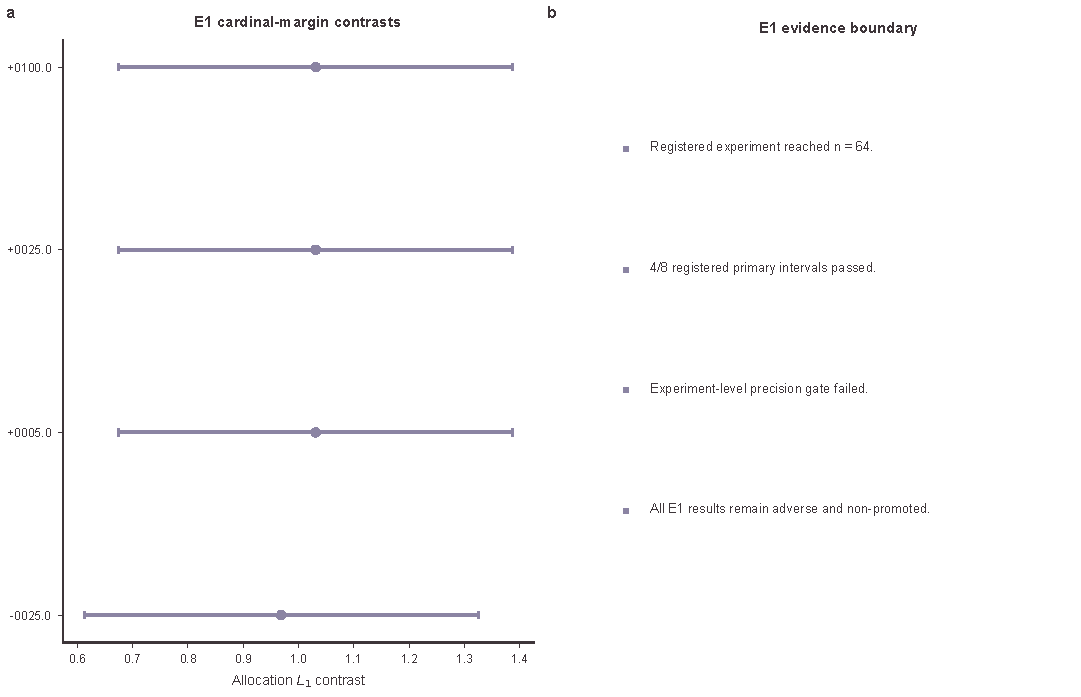
\includegraphics[width=\textwidth]{../figures/stage_ii/supplementary/FigureS1.pdf}
\caption{\textbf{Complete precision-gate ledger.} Final sequential outcomes for E1--E6. Only E2 and E6 pass every registered primary interval; failed experiments reach $n=64$ and remain non-promoted.}
\label{fig:s1}
\end{figure}

\subsection{E2 operational intervention family}
E2 holds the profit law, external corn-over-soybean ranking and deterministic selection rule fixed. The base cell has no budget, rotation, contract or corn-cap intervention. Factorial cells switch budget, rotation and contract indicators; a separate corn-bound anchor supplies an explicit bound mechanism. The expected-profit base selects corn share 1. Contract or rotation displacement caps corn at 0.45 and requires soybean share 0.55. The tight budget selects corn 0.318 and soybeans 0.682. Winter wheat remains zero in these constructed cells.

Each of the eight factorial contrasts reports allocation $L_1$ change, expected-profit change and selected-reversal change, giving \EtwoIntervals{} registered primary intervals. Every interval passes. The selected-reversal change is one with a multiplicity-adjusted lower bound of 0.628; the continuous allocation differences are deterministic conditional on the registered cell. The optimal-face audit verifies possible, selected and universal reversal together. The mechanism labels distinguish direct forcing, marginal pressure and inactive-in-cell restrictions; a named restriction can be present without being the active marginal term.

\subsection{E6 information--flexibility family}
E6 computes four optimized values in each constructive environment: uninformative/restricted, informative/restricted, uninformative/flexible and informative/flexible. The interaction is
\begin{equation}
\Delta_{I\times F}=[V(I,F)-V(U,F)]-[V(I,R)-V(U,R)].
\end{equation}
The specialization-unlocks construction gives \EsixPositive{} [\EsixPositiveLow{}, \EsixPositiveHigh{}]. The robust-option construction gives \EsixSubstitution{} [\EsixSubstitutionLow{}, \EsixSubstitutionHigh{}]. The dominated-option construction gives exactly \EsixNull{}. All three family-wise intervals pass at $n=\EsixReplications{}$. Ignore-signal policies reproduce uninformed values, and deterministic signal garbling cannot increase the optimized value under the registered comparison.

\subsection{Adverse experiments and infeasibility}
E1 tests margin-driven reversal, E3 the CVaR frontier, E4 dependence intensity within named families and E5 cross-law misspecification. Each has at least one registered primary interval that fails at $n=64$, so all four remain adverse regardless of the sign or apparent precision of individual rows. The failure may arise from interval width, insufficient finite observations after registered infeasibility, or both.

There are \RegisteredInfeasible{} registered infeasible rows: 192 are designed E3 frontier cases and 14 are certified E4/E5 cases. Every row has a reason and remains in the ledger. No solver failure remains unexplained after excluding registered infeasibility, and no feasible-only subset is used for a positive claim.

\begin{figure}[t]
\centering
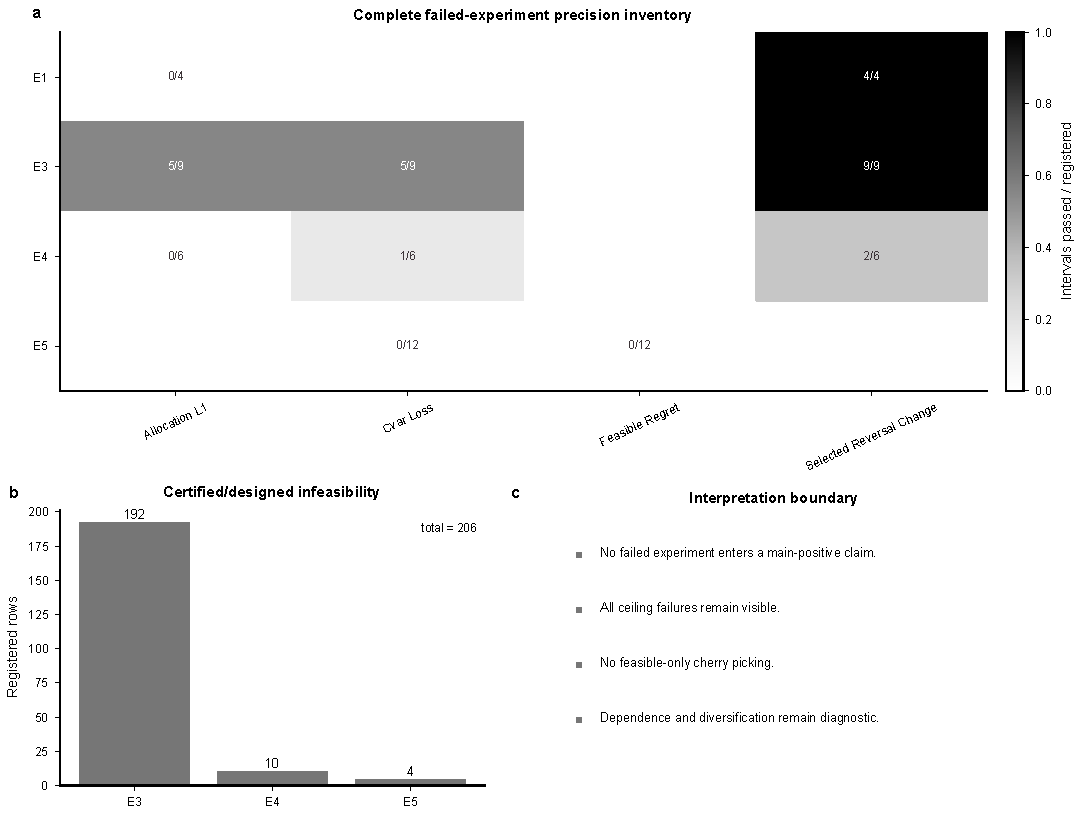
\includegraphics[width=\textwidth]{../figures/stage_ii/supplementary/FigureS2.pdf}
\caption{\textbf{Complete adverse and infeasible inventory.} Failed E1, E3, E4 and E5 estimands are shown with every \RegisteredInfeasible{} registered infeasible row (192 designed E3 rows and 14 certified E4/E5 rows). No feasible-only filtering enters a positive claim.}
\label{fig:s2}
\end{figure}

\subsection{Optimal faces, KKT checks and attribution closure}
The optimal-face audit fixes the primary objective within tolerance and minimizes and maximizes each relevant acreage gap. It thereby distinguishes possible, universal and selected reversal instead of treating one solver vertex as the entire solution set. Direct loss-CVaR is recomputed from optimized scenario losses and compared with the auxiliary value. Tail weights, stationarity, complementarity and primal feasibility are evaluated independently.

Reverse-order replay passes \ReplayPasses{}/\ReplayTotal{} registered checks and solver-method sensitivity passes \SolverPasses{}/\SolverTotal{}. The maximum KKT stationarity residual is $\KKTResidual$. For M0--M4 attribution, all coalitions of the margins, operations, risk and dependence blocks are solved. Shapley contributions sum to the full-minus-base change with maximum efficiency residual $\ShapleyResidual$.

\begin{figure}[t]
\centering
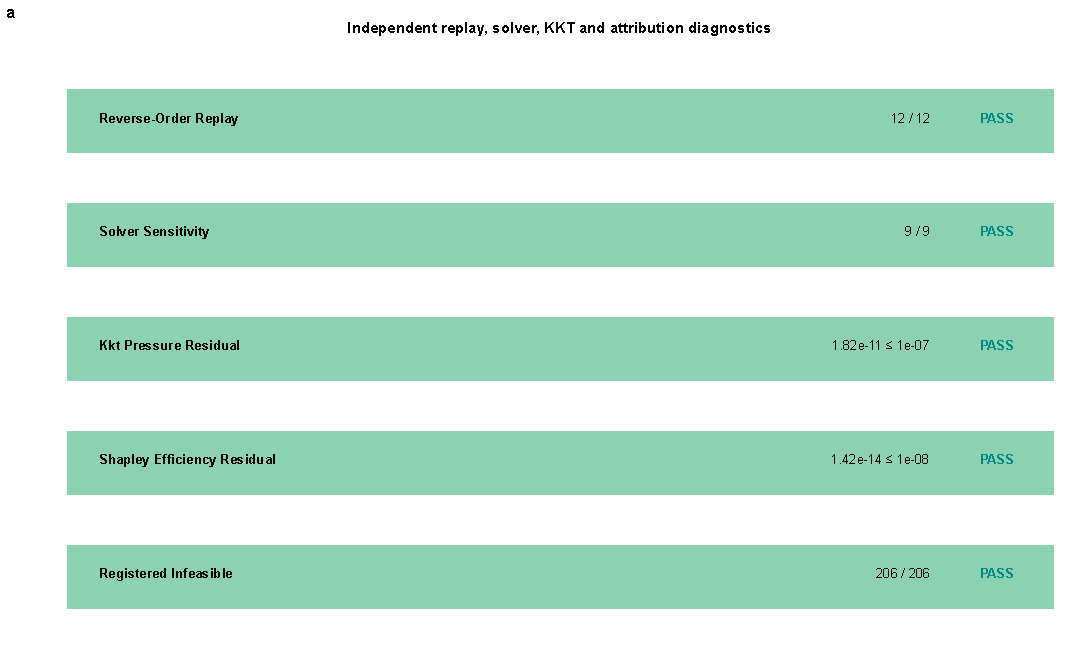
\includegraphics[width=\textwidth]{../figures/stage_ii/supplementary/FigureS3.pdf}
\caption{\textbf{Numerical diagnostics.} Reverse-order replay passes \ReplayPasses{}/\ReplayTotal{}, solver sensitivity passes \SolverPasses{}/\SolverTotal{}, the maximum KKT residual is $\KKTResidual$, and the maximum Shapley efficiency residual is $\ShapleyResidual$.}
\label{fig:s3}
\end{figure}

Sequential block paths can differ even when their endpoint is identical. Figure~\ref{fig:s4} therefore reports each block's contribution range over every registered order, with dots for order means. The all-subset Shapley value is the symmetric average of marginal contributions; it is an accounting allocation over the closed model domain, not a causal decomposition.

\begin{figure}[t]
\centering
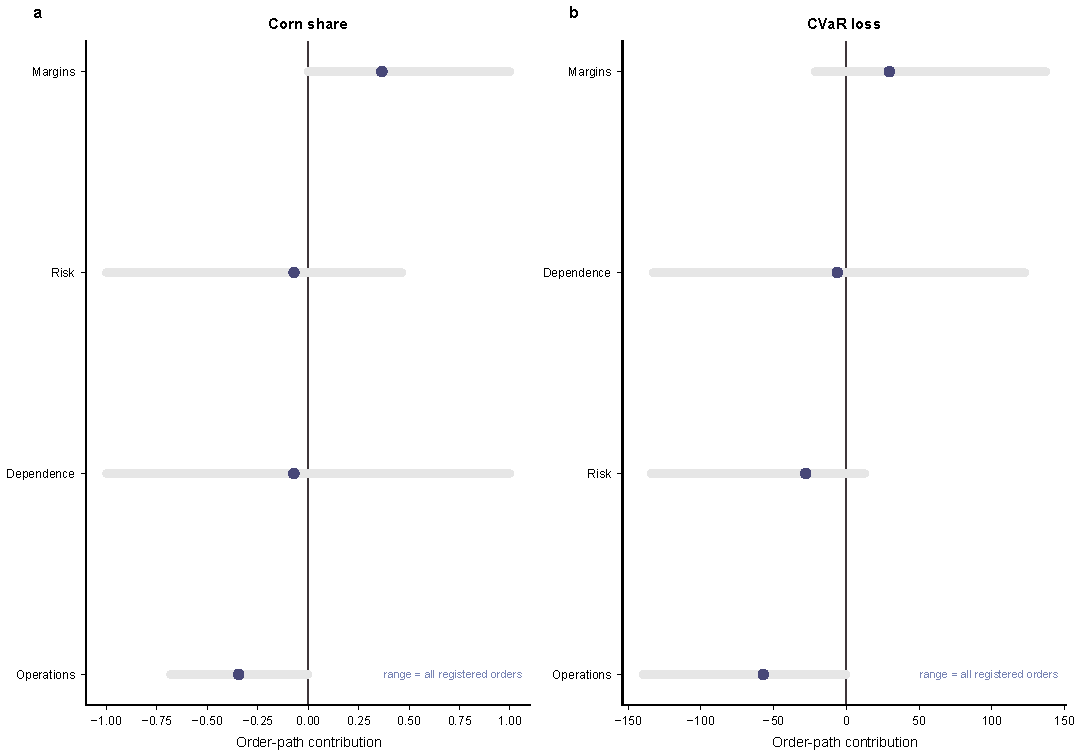
\includegraphics[width=\textwidth]{../figures/stage_ii/supplementary/FigureS4.pdf}
\caption{\textbf{Attribution order sensitivity.} Ranges cover all registered block orders and dots show order means. The display exposes path dependence rather than assigning causal meaning to one ordering.}
\label{fig:s4}
\end{figure}
